\section{B*-tree}
    \textit{Об этом дереве очень мало статей/лекций/документов, поэтому в этом разделе представленно максимальное количество информации, которую я смогла найти} \par
    Распространённая модификация B-дерева, в которой каждый внутренний узел должен быть заполнен как минимум на две трети, а не наполовину, как в случае со стандартным B-деревом. \par
    Алгоритм хранит интервалы для узлов дерева, а не точные значения. Листы можно искать до тех, пор пока одни из узлов верхнего уровня не будут иметь нужный интервал. Если интервалы неверны, то дерево может быть не в состоянии найти правильный путь, однако, на практике алгоритм достаточно устойчив к ошибкам.\par
    В отличие от B+-деревьев, узел не разбивается на 2 узла, если полностью заполнен. Вместо этого ищется место в существующем соседнем узле, и только после того, как оба узла будут заполнены, они разделяются на три узла. \par
    B*-деревья предложили Рудольф Байер и Эдвард МакКрейт, изучавшие проблему компактности B-деревьев. B*-дерево относительно компактнее, так как каждый узел используется полнее. В остальном же этот вид деревьев не отличается от простого B-дерева.
    \par
    B*-дерево порядка m – это дерево поиска, которое либо пусто, либо удовлетворяет трем свойствам:
    \par
    \begin{enumerate}
        \item Корень имеет минимум два и максимум ((2m-2)/3)+1 потомок 
        \item Остальные внутренние узлы имеют минимальный уровень ((2m-1)/3) и максимальное количество дочерних узлов m 
        \item Все внешние узлы находятся на одном уровне
    \end{enumerate}
    \newpage
    \subsection{Уникальные части алгоритма вставки В*-дерева:}
    \begin{enumerate}
        \item При вставке в полный листовой узел (не корень) и который имеет полный правый родственный элемент (и чей родитель имеет хотя бы один свободный ключ):
        \begin{itemize}
            \item Возьмем массив, состоящий из ключей «m-1» полного листового узла, родительского ключа этого узла, нового ключа, который нужно вставить, и ключей «m-1» его правого брата (всего m-1+1+1+m-1 = 2m ключей) 
            \item Сортировать эти ключи 
            \item Создать три новых узла:
            \begin{enumerate}
                \item P – чьи ключи являются первыми (2m-2)/3 элементами массива. Элемент с этим индексом хранится как «parent1»
                \item Q – чьи ключи являются следующими (2m-1)/3 элементами массива. Элемент с индексом (4m)/3 хранится как«parent2»
                \item К – чьи ключи являются последними (2m)/3 элементами массива после «parent2»
            \end{enumerate}
            \item Значение ключа в родительском листе, указывающего на этот лист, должно быть заменено на «parent1»
            \item Если родительский ключ имеет соседние ключи, их следует сдвинуть вправо. В оставшемся месте поместите «psrent2»
            \item P,q,r должны быть сделаны дочерними ключами «parent1» и «parent2» (если они являются первыми двумя ключами в род узле), иначе должны быть сделаны дочерними ключами перед parent1, parent2 соответственно
            \begin{center}
                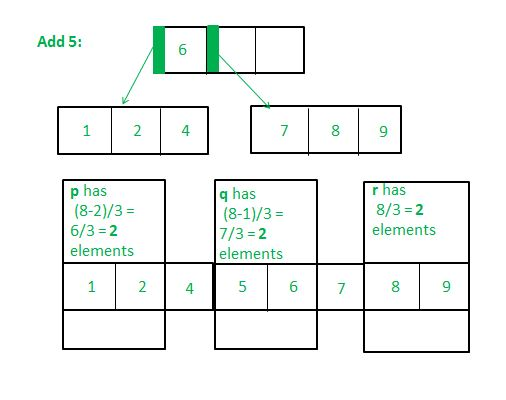
\includegraphics[width=0.7\linewidth]{gfg16.jpg} \par
            \end{center}
            \newpage
            \item При вставке в полный конечный узел (не корень) с пустым или неполным правым родственным элементом: Необходимо сдвинуть последний элемент текущего узла на позицию родителя, сдвинуть все ключи в правом соседнем элементе вправо и вставить предыдущего родителя. Использовать пробел в своем собственном узле, чтобы изменить порядок и вписать новый ключ.
            \begin{center}
                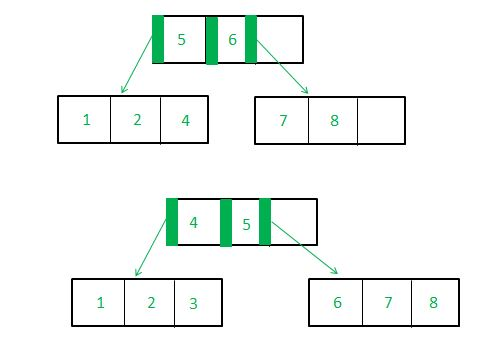
\includegraphics[width=0.6\linewidth]{gfg32.jpg} \par
            \end{center}
            \item Остальные случаи такие же, как и для В-деревьев

        \end{itemize}
    \end{enumerate}
    Преимущество использования В*-деревьев по сравнению с В-деревьями заключается в уникальной функции, называемой разделением «два к трем». Таким образом, минимальное количество ключей в каждом узле составляет не половину максимального, а две трети от него, что делает данные гораздо более компактными. Однако, недостатком этого является сложная операция удаления. \par
    Трудность в практической реализации В*-дерева объясняет почему он используется не так часто, как его аналоги.\par
    Этот термин в целом не используется сегодня, поскольку внедрение никогда не рассматривалось положительно сообществом информатики в целом; большинство людей используют "В-дерево" в общем плане для обозначения всех вариаций и усовершенствований структуры базовых данных. \par
    \newpage
    
